
    \documentclass[10pt,a4paper,twocolumn]{article}
    \usepackage[margin=1.8cm]{geometry}
    \usepackage{booktabs}
    \usepackage{graphicx}
    \usepackage{xcolor}
    \usepackage{hyperref}
    \usepackage{eurosym}
    \usepackage[small]{titlesec}
    \usepackage[T1]{fontenc}
    \setlength{\parindent}{0pt}
    \setlength{\parskip}{0.4em}

    \title{\textbf{AutoResearcher2: Research Progress Memo}\\[0.3em]
           \large v4.8 --- Generator-Critic Pipeline}
    \author{autoresearcher2 (autonomous)}
    \date{2026-03-15 20:28}

    \begin{document}
    \maketitle
    \thispagestyle{empty}

    \section*{Executive Summary}

    An autonomous research agent, starting with zero domain knowledge,
    designed and executed \textbf{77} GPU experiments
    across 2 projects,
    costing \textbf{\euro{}0.20} in electricity
    (0.715 kWh). 

    Through a generator-critic pipeline with an evolving world model,
    the system developed \textbf{49 explicit beliefs}
    about how training parameters interact --- each with a confidence score,
    supporting evidence, and natural language explanation.

    All results are exploratory (single-seed, no repetitions).
    The value is not in any individual finding, but in the agent's ability
    to build and communicate a structured understanding autonomously.

    \smallskip
    \noindent\textit{Source:} \url{https://github.com/erikdebruijn/autoresearcher2}

    \subsection*{Glossary}
    \small

    \textbf{val\_bpb} --- validation bits-per-byte; lower = better language model.

    \textbf{mean\_reward} --- average game score; higher = better agent.

    \textbf{DEPTH} --- number of transformer layers (model capacity).

    \textbf{MATRIX\_LR} --- learning rate for the main weight matrices.

    \textbf{WEIGHT\_DECAY} --- regularization strength (prevents overfitting).

    \textbf{Confidence} --- heuristic 0--1 score assigned by the LLM based on evidence count and consistency. Not a calibrated probability; treat as a ranking signal.

    \textbf{Belief} --- an LLM-generated claim about the domain, updated after each experiment. May mix observation and inference.

    \textbf{Tension} --- an open question the agent has identified but not yet resolved.
    \normalsize

    \section{Projects}


\subsection{NanoGPT}

\textbf{Target:} minimize \texttt{val\_bpb} \\
\textbf{Runs:} 51 successful, 20 failed \\
\textbf{World model:} v102 --- 40 beliefs, 11 tensions \\
\textbf{Cost:} 0.671 kWh, \euro{}0.18, 4.6 hours wall time

\subsubsection*{Best result}
\texttt{val\_bpb} = \textbf{1.036205} at run 49 (config\_change) \\
Config: \texttt{DEPTH=8, MATRIX\_LR=0.03, WEIGHT\_DECAY=0.1, batch\_size=64}

\begin{figure}[h]
\centering
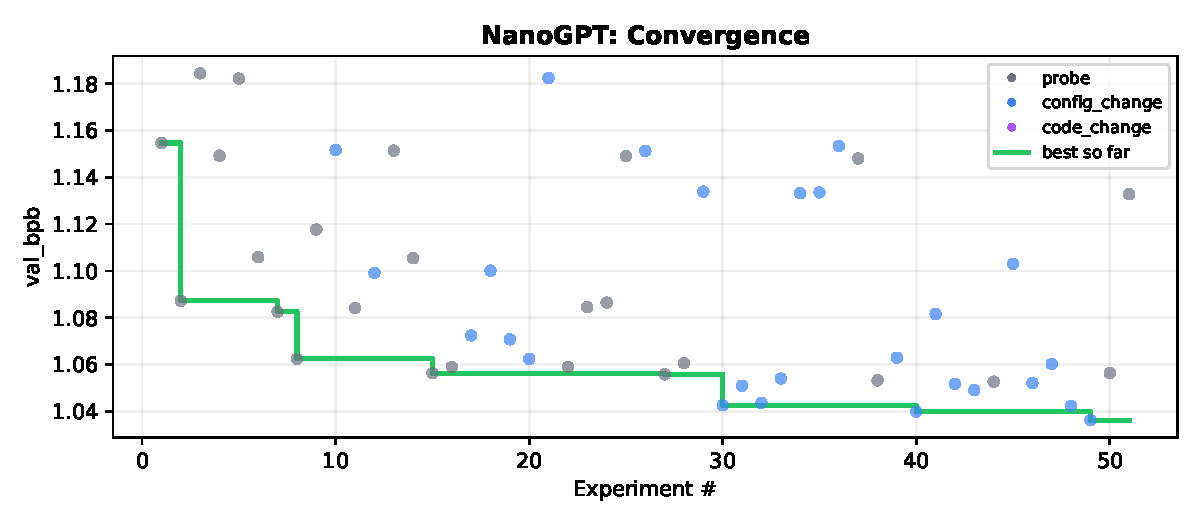
\includegraphics[width=\columnwidth]{figures/nanogpt_convergence.pdf}
\caption{NanoGPT: convergence over 51 experiments. Green line = cumulative best.}
\end{figure}

\begin{figure}[h]
\centering
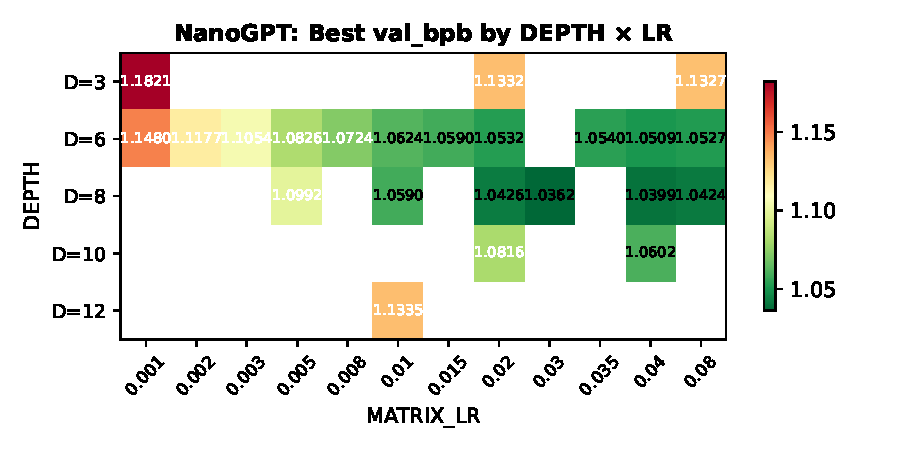
\includegraphics[width=0.85\columnwidth]{figures/nanogpt_heatmap.pdf}
\caption{Best val\_bpb per DEPTH $\times$ MATRIX\_LR cell. Lower (green) is better.}
\end{figure}

\subsubsection*{Key beliefs}
\begin{enumerate}
\small
  \item \textbf{[0.99]} The training system runs beyond the configured num\_steps (1000 requested, 2395 actual), likely completing full epochs over the data
  \item \textbf{[0.99]} The training infrastructure has a fragile dependency on a cached tokenizer file at /home/autoresearcher/.cache/autoresearch/tokenizer/tokenizer.pkl. If this file is missing or the 
  \item \textbf{[0.98]} Peak VRAM for DEPTH=6 is \textasciitilde{}14 GB regardless of whether batch\_size is 64 or 128, suggesting model parameters dominate memory usage over batch size in this range
  \item \textbf{[0.97]} Peak VRAM for DEPTH=8 with batch\_size=64 is \textasciitilde{}23.5 GB, roughly 1.7x the \textasciitilde{}14 GB used by DEPTH=6 configurations
  \item \textbf{[0.97]} The training system processes \textasciitilde{}131K tokens per step regardless of batch\_size (64 or 128) and depth (6 or 8), suggesting a fixed token-per-step budget. This explains why deeper/slow
  \item[] \textit{... and 35 more beliefs}
\end{enumerate}

\subsubsection*{Open questions}
\begin{itemize}
\small
  \item Only one data point establishes the depth-6 baseline; unclear whether this is near-optimal or far from optimal for this param count and token budget
  \item The num\_steps parameter appears ignored by the training system (400 requested, 2463 run). If this is epoch-based, the 'num\_steps' intervention spec may not control training duratio
  \item DEPTH=8 (67.6M params) achieves val\_bpb=1.099, which is WORSE than the best DEPTH=6 result (35.8M params, val\_bpb=1.084) despite nearly 2x parameters. However, this comparison is h
\end{itemize}

\subsubsection*{Measured cost per experiment}
\begin{table}[h]
\centering
\small
\begin{tabular}{lrrr}
\toprule
Type & Wall time (s) & Energy (Wh) & Cost (\euro{{}}) \\
\midrule
  config\_change & 320 & 29.8 & 0.0086 \\
  probe & 320 & 29.1 & 0.0084 \\
\bottomrule
\end{tabular}
\end{table}

\subsection{Atari Breakout}

\textbf{Target:} maximize \texttt{mean\_reward} \\
\textbf{Runs:} 6 successful, 0 failed \\
\textbf{World model:} v97 --- 9 beliefs, 2 tensions \\
\textbf{Cost:} 0.045 kWh, \euro{}0.01, 0.4 hours wall time

\subsubsection*{Best result}
\texttt{mean\_reward} = \textbf{3.600000} at run 2 (probe) \\
Config: \texttt{total\_timesteps=50000, learning\_rate=0.00025, n\_envs=4}

\begin{figure}[h]
\centering
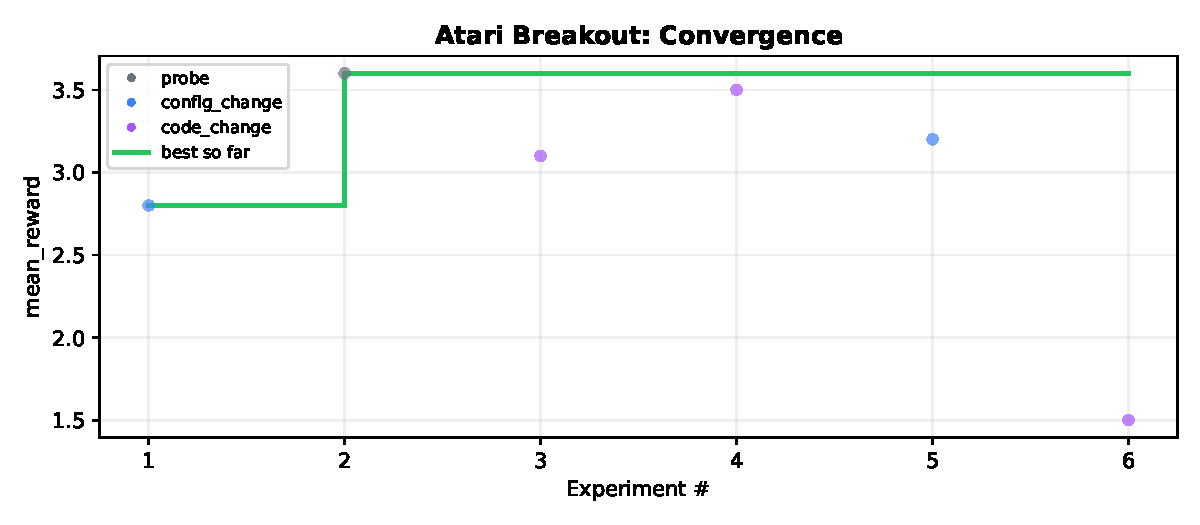
\includegraphics[width=\columnwidth]{figures/atari_breakout_convergence.pdf}
\caption{Atari Breakout: convergence over 6 experiments. Green line = cumulative best.}
\end{figure}

\subsubsection*{Key beliefs}
\begin{enumerate}
\small
  \item \textbf{[0.75]} The agent is in early training — explained\_variance rose from 0.758 to 0.845 near end of run, suggesting the value function is still improving
  \item \textbf{[0.60]} Entropy loss decreased from -0.282 to -0.267 over final iterations, indicating policy is still exploring but gradually specializing
  \item \textbf{[0.55]} PPO with lr=0.00025, 4 envs, 200k timesteps yields mean\_reward=2.8 (std=1.6) on this Atari task
  \item \textbf{[0.50]} The lr decay schedule produces substantially lower entropy (-0.21) and very low clip\_fraction (\textasciitilde{}0.004-0.007), indicating a more converged but potentially prematurely specialized po
  \item \textbf{[0.50]} Reward shaping (survival\_bonus=0.01, life\_loss\_penalty=-1.0) with PPO at lr=2.5e-4 and 200k timesteps yields mean\_reward=1.5 (std=1.2), substantially worse than the unshaped baseli
  \item[] \textit{... and 4 more beliefs}
\end{enumerate}

\subsubsection*{Open questions}
\begin{itemize}
\small
  \item The lr decay schedule (1e-3$\to$1e-5) achieved mean\_reward=3.5 vs fixed lr=2.5e-4's 2.8. However, the decay schedule also drove entropy much lower (-0.21 vs -0.267) and clip\_fraction n
  \item Reward shaping (survival bonus + life-loss penalty) was intended to accelerate early learning but reduced mean\_reward from 2.8 to 1.5 — a 46\% drop. The value function learned the s
\end{itemize}

\subsubsection*{Measured cost per experiment}
\begin{table}[h]
\centering
\small
\begin{tabular}{lrrr}
\toprule
Type & Wall time (s) & Energy (Wh) & Cost (\euro{{}}) \\
\midrule
  config\_change\_200k\_steps & 252 & 7.0 & 0.0018 \\
  reward\_shaping\_200k\_steps & 271 & 7.1 & 0.0018 \\
\bottomrule
\end{tabular}
\end{table}


    \section{Method}

    \subsection*{Pipeline}
    The system follows an OODA loop:
    \textbf{Orient} (update world model from latest result) $\to$
    \textbf{Generate} (LLM proposes 5 experiments, reasoning from epistemic intent) $\to$
    \textbf{Critique} (LLM ranks by information value, selects top 3) $\to$
    \textbf{Execute} (run on GPU, parse metrics, feed back).

    Each proposal follows: epistemic intent $\to$ rationale $\to$
    expected learning $\to$ intervention $\to$ cost estimate.
    This ensures experiments are designed to \emph{learn something regardless of outcome}.

    \subsection*{Experiment protocol}
    Each run trains a single model configuration to completion (single seed, no repetition).
    The agent controls hyperparameters (config\_change) or full training scripts (code\_change).
    A run is ``successful'' if it completes without error and produces a metric;
    ``failed'' runs (OOM, script errors) still inform the world model.
    Energy consumption is measured per-GPU via nvidia-smi polling at 1\,Hz.

    \subsection*{Confidence scores}
    Confidence values (0--1) are assigned by the LLM during world-model updates.
    They reflect evidence count and internal consistency, not frequentist probabilities.
    They are useful for ranking beliefs but should not be interpreted as calibrated.

    \section{Limitations}

    \begin{itemize}
        \item \textbf{Single seed}: no statistical significance; any result could be noise
        \item \textbf{No ablation}: the LLM's contribution vs.\ simpler optimization is untested
        \item \textbf{Hardware-specific}: all runs on one GPU (RTX PRO 6000, 96\,GB VRAM)
        \item \textbf{Beliefs mix observation and inference}: claims like ``X explains Y''
              are the agent's interpretation, not proven causal links
        \item \textbf{Exploratory}: this memo reports what the agent found, not what is established
    \end{itemize}

    \end{document}
